\documentclass[]{article}
\usepackage{lmodern}
\usepackage{amssymb,amsmath}
\usepackage{ifxetex,ifluatex}
\usepackage{fixltx2e} % provides \textsubscript
\ifnum 0\ifxetex 1\fi\ifluatex 1\fi=0 % if pdftex
  \usepackage[T1]{fontenc}
  \usepackage[utf8]{inputenc}
\else % if luatex or xelatex
  \ifxetex
    \usepackage{mathspec}
  \else
    \usepackage{fontspec}
  \fi
  \defaultfontfeatures{Ligatures=TeX,Scale=MatchLowercase}
\fi
% use upquote if available, for straight quotes in verbatim environments
\IfFileExists{upquote.sty}{\usepackage{upquote}}{}
% use microtype if available
\IfFileExists{microtype.sty}{%
\usepackage{microtype}
\UseMicrotypeSet[protrusion]{basicmath} % disable protrusion for tt fonts
}{}
\usepackage[margin=1in]{geometry}
\usepackage{hyperref}
\hypersetup{unicode=true,
            pdftitle={Assignment 2},
            pdfborder={0 0 0},
            breaklinks=true}
\urlstyle{same}  % don't use monospace font for urls
\usepackage{color}
\usepackage{fancyvrb}
\newcommand{\VerbBar}{|}
\newcommand{\VERB}{\Verb[commandchars=\\\{\}]}
\DefineVerbatimEnvironment{Highlighting}{Verbatim}{commandchars=\\\{\}}
% Add ',fontsize=\small' for more characters per line
\usepackage{framed}
\definecolor{shadecolor}{RGB}{248,248,248}
\newenvironment{Shaded}{\begin{snugshade}}{\end{snugshade}}
\newcommand{\AlertTok}[1]{\textcolor[rgb]{0.94,0.16,0.16}{#1}}
\newcommand{\AnnotationTok}[1]{\textcolor[rgb]{0.56,0.35,0.01}{\textbf{\textit{#1}}}}
\newcommand{\AttributeTok}[1]{\textcolor[rgb]{0.77,0.63,0.00}{#1}}
\newcommand{\BaseNTok}[1]{\textcolor[rgb]{0.00,0.00,0.81}{#1}}
\newcommand{\BuiltInTok}[1]{#1}
\newcommand{\CharTok}[1]{\textcolor[rgb]{0.31,0.60,0.02}{#1}}
\newcommand{\CommentTok}[1]{\textcolor[rgb]{0.56,0.35,0.01}{\textit{#1}}}
\newcommand{\CommentVarTok}[1]{\textcolor[rgb]{0.56,0.35,0.01}{\textbf{\textit{#1}}}}
\newcommand{\ConstantTok}[1]{\textcolor[rgb]{0.00,0.00,0.00}{#1}}
\newcommand{\ControlFlowTok}[1]{\textcolor[rgb]{0.13,0.29,0.53}{\textbf{#1}}}
\newcommand{\DataTypeTok}[1]{\textcolor[rgb]{0.13,0.29,0.53}{#1}}
\newcommand{\DecValTok}[1]{\textcolor[rgb]{0.00,0.00,0.81}{#1}}
\newcommand{\DocumentationTok}[1]{\textcolor[rgb]{0.56,0.35,0.01}{\textbf{\textit{#1}}}}
\newcommand{\ErrorTok}[1]{\textcolor[rgb]{0.64,0.00,0.00}{\textbf{#1}}}
\newcommand{\ExtensionTok}[1]{#1}
\newcommand{\FloatTok}[1]{\textcolor[rgb]{0.00,0.00,0.81}{#1}}
\newcommand{\FunctionTok}[1]{\textcolor[rgb]{0.00,0.00,0.00}{#1}}
\newcommand{\ImportTok}[1]{#1}
\newcommand{\InformationTok}[1]{\textcolor[rgb]{0.56,0.35,0.01}{\textbf{\textit{#1}}}}
\newcommand{\KeywordTok}[1]{\textcolor[rgb]{0.13,0.29,0.53}{\textbf{#1}}}
\newcommand{\NormalTok}[1]{#1}
\newcommand{\OperatorTok}[1]{\textcolor[rgb]{0.81,0.36,0.00}{\textbf{#1}}}
\newcommand{\OtherTok}[1]{\textcolor[rgb]{0.56,0.35,0.01}{#1}}
\newcommand{\PreprocessorTok}[1]{\textcolor[rgb]{0.56,0.35,0.01}{\textit{#1}}}
\newcommand{\RegionMarkerTok}[1]{#1}
\newcommand{\SpecialCharTok}[1]{\textcolor[rgb]{0.00,0.00,0.00}{#1}}
\newcommand{\SpecialStringTok}[1]{\textcolor[rgb]{0.31,0.60,0.02}{#1}}
\newcommand{\StringTok}[1]{\textcolor[rgb]{0.31,0.60,0.02}{#1}}
\newcommand{\VariableTok}[1]{\textcolor[rgb]{0.00,0.00,0.00}{#1}}
\newcommand{\VerbatimStringTok}[1]{\textcolor[rgb]{0.31,0.60,0.02}{#1}}
\newcommand{\WarningTok}[1]{\textcolor[rgb]{0.56,0.35,0.01}{\textbf{\textit{#1}}}}
\usepackage{graphicx,grffile}
\makeatletter
\def\maxwidth{\ifdim\Gin@nat@width>\linewidth\linewidth\else\Gin@nat@width\fi}
\def\maxheight{\ifdim\Gin@nat@height>\textheight\textheight\else\Gin@nat@height\fi}
\makeatother
% Scale images if necessary, so that they will not overflow the page
% margins by default, and it is still possible to overwrite the defaults
% using explicit options in \includegraphics[width, height, ...]{}
\setkeys{Gin}{width=\maxwidth,height=\maxheight,keepaspectratio}
\IfFileExists{parskip.sty}{%
\usepackage{parskip}
}{% else
\setlength{\parindent}{0pt}
\setlength{\parskip}{6pt plus 2pt minus 1pt}
}
\setlength{\emergencystretch}{3em}  % prevent overfull lines
\providecommand{\tightlist}{%
  \setlength{\itemsep}{0pt}\setlength{\parskip}{0pt}}
\setcounter{secnumdepth}{0}
% Redefines (sub)paragraphs to behave more like sections
\ifx\paragraph\undefined\else
\let\oldparagraph\paragraph
\renewcommand{\paragraph}[1]{\oldparagraph{#1}\mbox{}}
\fi
\ifx\subparagraph\undefined\else
\let\oldsubparagraph\subparagraph
\renewcommand{\subparagraph}[1]{\oldsubparagraph{#1}\mbox{}}
\fi

%%% Use protect on footnotes to avoid problems with footnotes in titles
\let\rmarkdownfootnote\footnote%
\def\footnote{\protect\rmarkdownfootnote}

%%% Change title format to be more compact
\usepackage{titling}

% Create subtitle command for use in maketitle
\newcommand{\subtitle}[1]{
  \posttitle{
    \begin{center}\large#1\end{center}
    }
}

\setlength{\droptitle}{-2em}

  \title{Assignment 2}
    \pretitle{\vspace{\droptitle}\centering\huge}
  \posttitle{\par}
    \author{}
    \preauthor{}\postauthor{}
    \date{}
    \predate{}\postdate{}
  

\begin{document}
\maketitle

\begin{Shaded}
\begin{Highlighting}[]
\KeywordTok{library}\NormalTok{(tidyverse)}
\end{Highlighting}
\end{Shaded}

\begin{enumerate}
\def\labelenumi{\arabic{enumi}.}
\tightlist
\item
  For the data matrix below:
\end{enumerate}

\begin{Shaded}
\begin{Highlighting}[]
\NormalTok{x <-}\StringTok{ }\KeywordTok{matrix}\NormalTok{(}\KeywordTok{c}\NormalTok{(}\DecValTok{4}\NormalTok{ ,}\DecValTok{1}\NormalTok{,}\OperatorTok{-}\DecValTok{1}\NormalTok{,}\OperatorTok{-}\DecValTok{3}\NormalTok{,}\DecValTok{1}\NormalTok{, }\DecValTok{2}\NormalTok{,}\DecValTok{0}\NormalTok{,}\OperatorTok{-}\DecValTok{1}\NormalTok{,}\DecValTok{5}\NormalTok{,}\OperatorTok{-}\DecValTok{1}\NormalTok{), }\DataTypeTok{nrow=}\DecValTok{5}\NormalTok{)}
\NormalTok{x}
\end{Highlighting}
\end{Shaded}

\begin{verbatim}
##      [,1] [,2]
## [1,]    4    2
## [2,]    1    0
## [3,]   -1   -1
## [4,]   -3    5
## [5,]    1   -1
\end{verbatim}

\begin{enumerate}
\def\labelenumi{(\alph{enumi})}
\tightlist
\item
  Calculate the sample variance-covariance matrix.
\end{enumerate}

\begin{Shaded}
\begin{Highlighting}[]
\KeywordTok{var}\NormalTok{(x)}
\end{Highlighting}
\end{Shaded}

\begin{verbatim}
##       [,1]  [,2]
## [1,]  6.80 -2.25
## [2,] -2.25  6.50
\end{verbatim}

\begin{enumerate}
\def\labelenumi{(\alph{enumi})}
\setcounter{enumi}{1}
\tightlist
\item
  Calculate the correlation matrix.
\end{enumerate}

\begin{Shaded}
\begin{Highlighting}[]
\KeywordTok{cor}\NormalTok{(x)}
\end{Highlighting}
\end{Shaded}

\begin{verbatim}
##           [,1]      [,2]
## [1,]  1.000000 -0.338432
## [2,] -0.338432  1.000000
\end{verbatim}

\begin{enumerate}
\def\labelenumi{(\alph{enumi})}
\setcounter{enumi}{2}
\tightlist
\item
  Standardize the variables to have mean 0 and standard deviation 1.
\end{enumerate}

\begin{Shaded}
\begin{Highlighting}[]
\NormalTok{xs <-}\StringTok{ }\KeywordTok{scale}\NormalTok{(x)}
\NormalTok{xs}
\end{Highlighting}
\end{Shaded}

\begin{verbatim}
##            [,1]       [,2]
## [1,]  1.3805370  0.3922323
## [2,]  0.2300895 -0.3922323
## [3,] -0.5368755 -0.7844645
## [4,] -1.3038405  1.5689291
## [5,]  0.2300895 -0.7844645
## attr(,"scaled:center")
## [1] 0.4 1.0
## attr(,"scaled:scale")
## [1] 2.607681 2.549510
\end{verbatim}

\begin{enumerate}
\def\labelenumi{(\alph{enumi})}
\setcounter{enumi}{3}
\tightlist
\item
  In R find the eigenvectors of the correlation matrix of x.
\end{enumerate}

\begin{Shaded}
\begin{Highlighting}[]
\KeywordTok{t}\NormalTok{(xs)}\OperatorTok\NormalTok{(xs)}\OperatorTok{/}\NormalTok{(}\KeywordTok{nrow}\NormalTok{(xs) }\OperatorTok{-}\StringTok{ }\DecValTok{1}\NormalTok{)}
\end{Highlighting}
\end{Shaded}

\begin{verbatim}
##           [,1]      [,2]
## [1,]  1.000000 -0.338432
## [2,] -0.338432  1.000000
\end{verbatim}

\begin{Shaded}
\begin{Highlighting}[]
\KeywordTok{var}\NormalTok{(xs)}
\end{Highlighting}
\end{Shaded}

\begin{verbatim}
##           [,1]      [,2]
## [1,]  1.000000 -0.338432
## [2,] -0.338432  1.000000
\end{verbatim}

\begin{Shaded}
\begin{Highlighting}[]
\KeywordTok{eigen}\NormalTok{(}\KeywordTok{cor}\NormalTok{(x))}
\end{Highlighting}
\end{Shaded}

\begin{verbatim}
## eigen() decomposition
## $values
## [1] 1.338432 0.661568
## 
## $vectors
##            [,1]       [,2]
## [1,] -0.7071068 -0.7071068
## [2,]  0.7071068 -0.7071068
\end{verbatim}

\begin{enumerate}
\def\labelenumi{(\alph{enumi})}
\setcounter{enumi}{4}
\tightlist
\item
  Using prcomp() function, find the loadings for the principal
  components of x.
\end{enumerate}

\begin{Shaded}
\begin{Highlighting}[]
\KeywordTok{prcomp}\NormalTok{(x, }\DataTypeTok{scale =} \OtherTok{TRUE}\NormalTok{)}
\end{Highlighting}
\end{Shaded}

\begin{verbatim}
## Standard deviations (1, .., p=2):
## [1] 1.1569062 0.8133683
## 
## Rotation (n x k) = (2 x 2):
##             PC1       PC2
## [1,] -0.7071068 0.7071068
## [2,]  0.7071068 0.7071068
\end{verbatim}

\begin{enumerate}
\def\labelenumi{\arabic{enumi}.}
\setcounter{enumi}{1}
\tightlist
\item
  Body fat data. The data consists of observations taken on a sample of
  88 males. In this question you will look at PCA of the variables
  variables were measured:
\end{enumerate}

\begin{itemize}
\tightlist
\item
  Neck circumference (cm)
\item
  Abdomen circumference (cm)
\item
  Knee circumference (cm)
\item
  Ankle circumference (cm)
\end{itemize}

\begin{Shaded}
\begin{Highlighting}[]
\NormalTok{bodyfat <-}\StringTok{ }\KeywordTok{read.table}\NormalTok{(}\StringTok{"data/bodyfat.txt"}\NormalTok{, }\DataTypeTok{header =} \OtherTok{TRUE}\NormalTok{) }\OperatorTok\StringTok{ }
\StringTok{  }\KeywordTok{select}\NormalTok{(neck, abdomen, knee, ankle)}
\KeywordTok{head}\NormalTok{(bodyfat)}
\end{Highlighting}
\end{Shaded}

\begin{verbatim}
##   neck abdomen knee ankle
## 1 36.2    85.2 37.3  21.9
## 2 38.5    83.0 37.3  23.4
## 3 34.0    87.9 38.9  24.0
## 4 37.4    86.4 37.3  22.8
## 5 34.4   100.0 42.2  24.0
## 6 39.0    94.4 42.0  25.6
\end{verbatim}

Use pairs to construct a scatterplot matrix. Are there any outliers? If
so, which cases are they?

\begin{Shaded}
\begin{Highlighting}[]
\KeywordTok{pairs}\NormalTok{(bodyfat)}
\end{Highlighting}
\end{Shaded}

\begin{center}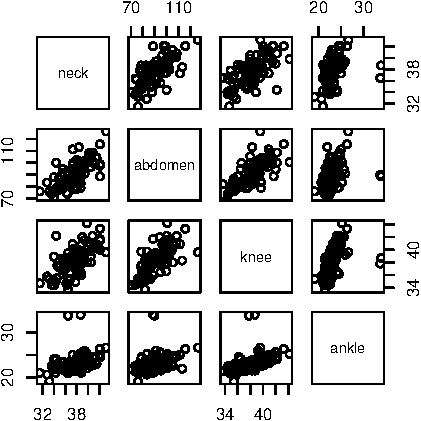
\includegraphics{sol_A2_files/figure-latex/unnamed-chunk-9-1} \end{center}

\begin{Shaded}
\begin{Highlighting}[]
\NormalTok{bodyfat }\OperatorTok\StringTok{ }\KeywordTok{filter}\NormalTok{(ankle }\OperatorTok{>}\StringTok{ }\DecValTok{30}\NormalTok{)}
\end{Highlighting}
\end{Shaded}

\begin{verbatim}
##   neck abdomen knee ankle
## 1 38.7    88.7 38.7  33.9
## 2 36.5    89.7 37.8  33.7
\end{verbatim}

\begin{quote}
There are two outliers with extreme ankle values, but non extreme values
on other variables. They are observations 31 and 84.
\end{quote}

\begin{enumerate}
\def\labelenumi{(\alph{enumi})}
\setcounter{enumi}{1}
\tightlist
\item
  Carry out a principal components analysis of the data. What percentage
  of the variability in the dataset is accounted for by the first
  component? What percentage of the variability in the dataset is
  accounted for by the first two components? Examine the scree diagram
  and comment. (You will find the code for the screeplot in h1code.R).
\end{enumerate}

\begin{Shaded}
\begin{Highlighting}[]
\NormalTok{scree_ggplot <-}\StringTok{ }\ControlFlowTok{function}\NormalTok{(p) \{}
\NormalTok{  e <-}\StringTok{ }\NormalTok{p}\OperatorTok{$}\NormalTok{sdev }\OperatorTok{^}\StringTok{ }\DecValTok{2}
\NormalTok{  df <-}\StringTok{ }\KeywordTok{data.frame}\NormalTok{(}\DataTypeTok{e =}\NormalTok{ e }\OperatorTok{/}\StringTok{ }\KeywordTok{sum}\NormalTok{(e), }\DataTypeTok{ind =} \DecValTok{1}\OperatorTok{:}\KeywordTok{length}\NormalTok{(e))}
\NormalTok{  df }\OperatorTok\StringTok{ }
\StringTok{    }\KeywordTok{ggplot}\NormalTok{(}\KeywordTok{aes}\NormalTok{(ind, e)) }\OperatorTok{+}
\StringTok{    }\KeywordTok{geom_line}\NormalTok{(}\DataTypeTok{linetype =} \StringTok{"dotted"}\NormalTok{, }\DataTypeTok{size =} \FloatTok{0.7}\NormalTok{) }\OperatorTok{+}
\StringTok{    }\KeywordTok{geom_point}\NormalTok{(}\DataTypeTok{colour =} \StringTok{"orange"}\NormalTok{, }\DataTypeTok{size =} \FloatTok{2.5}\NormalTok{) }\OperatorTok{+}\StringTok{ }
\StringTok{    }\KeywordTok{labs}\NormalTok{(}\DataTypeTok{x =} \StringTok{"Component number"}\NormalTok{, }\DataTypeTok{y =} \StringTok{"Variance proportion"}\NormalTok{, }
         \DataTypeTok{title =} \StringTok{"Scree plot"}\NormalTok{) }\OperatorTok{+}
\StringTok{    }\KeywordTok{theme_bw}\NormalTok{()}
\NormalTok{  \}}


\NormalTok{p <-}\StringTok{ }\KeywordTok{prcomp}\NormalTok{(bodyfat, }\DataTypeTok{scale =} \OtherTok{TRUE}\NormalTok{)}
\NormalTok{p}\OperatorTok{$}\NormalTok{rotation[,}\DecValTok{1}\OperatorTok{:}\DecValTok{2}\NormalTok{] }
\end{Highlighting}
\end{Shaded}

\begin{verbatim}
##               PC1         PC2
## neck    0.5283837  0.21938447
## abdomen 0.5351101  0.35203936
## knee    0.5460990  0.05660109
## ankle   0.3691120 -0.90814925
\end{verbatim}

\begin{Shaded}
\begin{Highlighting}[]
\KeywordTok{summary}\NormalTok{(p)}
\end{Highlighting}
\end{Shaded}

\begin{verbatim}
## Importance of components:
##                           PC1    PC2     PC3     PC4
## Standard deviation     1.6283 0.8731 0.58678 0.49183
## Proportion of Variance 0.6629 0.1906 0.08608 0.06047
## Cumulative Proportion  0.6629 0.8535 0.93953 1.00000
\end{verbatim}

\begin{Shaded}
\begin{Highlighting}[]
\KeywordTok{scree_ggplot}\NormalTok{(p)}
\end{Highlighting}
\end{Shaded}

\begin{center}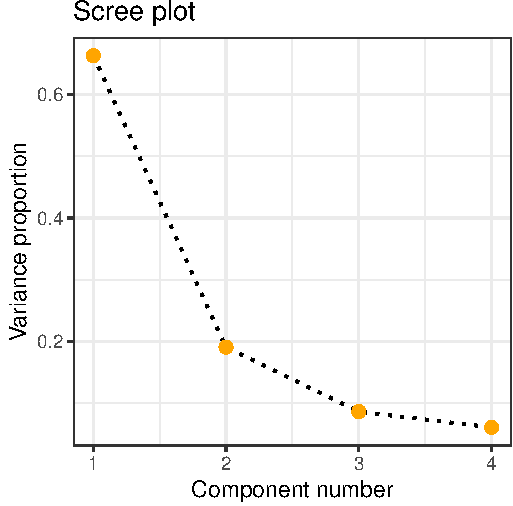
\includegraphics{sol_A2_files/figure-latex/unnamed-chunk-10-1} \end{center}

\(\approx\) 66\% of variability explained by the 1st PC, \(\approx\)
85\% by the first 2 PCs and \(\approx\) 94\% by the first 3 PCs.

\begin{enumerate}
\def\labelenumi{(\alph{enumi})}
\setcounter{enumi}{2}
\tightlist
\item
  What does the first component measure? the second component? Make a
  biplot to assist your interpretations. Are there any outliers? What
  can you say about the outliers from the plot?
\end{enumerate}

\begin{Shaded}
\begin{Highlighting}[]
\KeywordTok{biplot}\NormalTok{(p, }\DataTypeTok{scale =} \DecValTok{0}\NormalTok{, }\DataTypeTok{cex=}\KeywordTok{c}\NormalTok{(}\FloatTok{0.5}\NormalTok{, }\FloatTok{0.5}\NormalTok{), }\DataTypeTok{cex.axis =} \FloatTok{0.5}\NormalTok{)}
\end{Highlighting}
\end{Shaded}

\begin{center}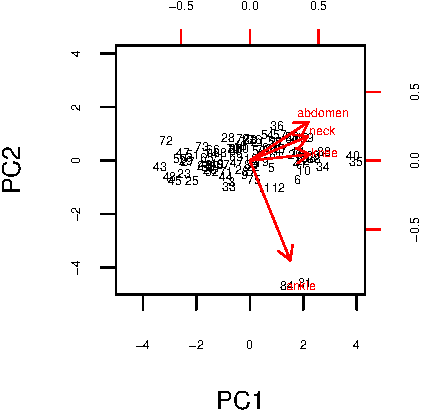
\includegraphics{sol_A2_files/figure-latex/unnamed-chunk-11-1} \end{center}

The first component is a weighted average of the variables. It is an
overall measure of size. The second component is a contrast of neck and
abdomen with ankle. It is a measure of the difference between top size
and ankle. The visible outliers are 84 and 31, with the big ankle
values.

\begin{enumerate}
\def\labelenumi{(\alph{enumi})}
\setcounter{enumi}{3}
\tightlist
\item
  Omiting any outliers identified, repeat parts (b) and (c).
\end{enumerate}

\begin{Shaded}
\begin{Highlighting}[]
\NormalTok{p <-}\StringTok{ }\KeywordTok{prcomp}\NormalTok{(bodyfat }\OperatorTok\StringTok{ }\KeywordTok{filter}\NormalTok{(ankle }\OperatorTok{<}\StringTok{ }\DecValTok{30}\NormalTok{), }\DataTypeTok{scale =} \OtherTok{TRUE}\NormalTok{)}
\NormalTok{p}\OperatorTok{$}\NormalTok{rotation[,}\DecValTok{1}\OperatorTok{:}\DecValTok{2}\NormalTok{]}
\end{Highlighting}
\end{Shaded}

\begin{verbatim}
##               PC1        PC2
## neck    0.5002906  0.3230518
## abdomen 0.5005250  0.5460175
## knee    0.5251301 -0.1447403
## ankle   0.4726758 -0.7593106
\end{verbatim}

\begin{Shaded}
\begin{Highlighting}[]
\KeywordTok{summary}\NormalTok{(p)}
\end{Highlighting}
\end{Shaded}

\begin{verbatim}
## Importance of components:
##                           PC1    PC2     PC3     PC4
## Standard deviation     1.7186 0.7186 0.58020 0.43962
## Proportion of Variance 0.7384 0.1291 0.08416 0.04832
## Cumulative Proportion  0.7384 0.8675 0.95168 1.00000
\end{verbatim}

\begin{Shaded}
\begin{Highlighting}[]
\KeywordTok{scree_ggplot}\NormalTok{(p)}
\end{Highlighting}
\end{Shaded}

\begin{center}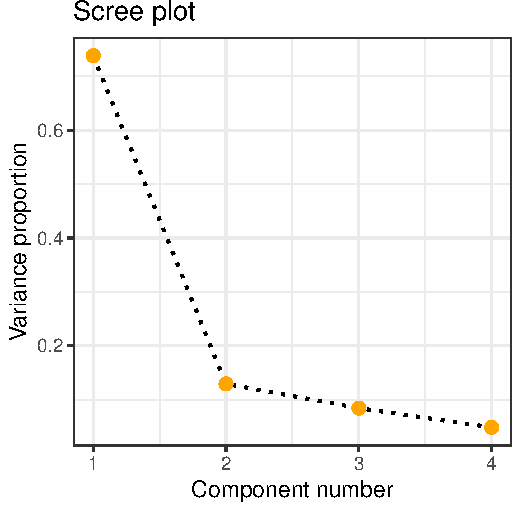
\includegraphics{sol_A2_files/figure-latex/unnamed-chunk-12-1} \end{center}

\begin{Shaded}
\begin{Highlighting}[]
\KeywordTok{biplot}\NormalTok{(p, }\DataTypeTok{scale=}\DecValTok{0}\NormalTok{, }\DataTypeTok{cex=}\KeywordTok{c}\NormalTok{(.}\DecValTok{5}\NormalTok{,.}\DecValTok{5}\NormalTok{), }\DataTypeTok{cex.axis=}\NormalTok{.}\DecValTok{5}\NormalTok{)}
\end{Highlighting}
\end{Shaded}

\begin{center}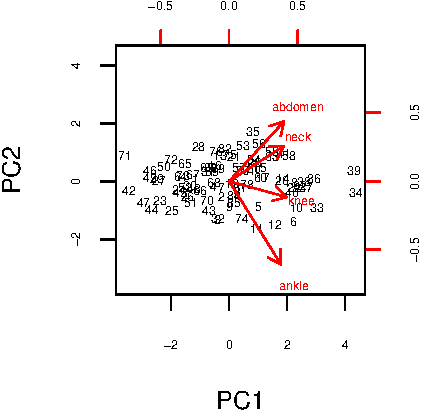
\includegraphics{sol_A2_files/figure-latex/unnamed-chunk-12-2} \end{center}

The first component is a weighted average of the variables. It is an
overall measure of size. The second component is a contrast of neck and
abdomen with knee and ankle. It is a measure of the difference between
top size and lower size. The high weight people stick out on the first
component, but are not that extreme.

\begin{enumerate}
\def\labelenumi{\arabic{enumi}.}
\setcounter{enumi}{2}
\tightlist
\item
  A 1902 study obtained measurements on seven physical characteristics
  for each of 3000 criminals. The seven variables measured were (1) head
  length (2) head breadth (3) face breadth (4) left finger length (5)
  left forearm length (6) left foot length (7) height. Using the
  correlation matrix given below, find the principal components of the
  data and interpret the results. What percentage of the variability in
  the dataset is accounted for by the first component? What percentage
  of the variability in the dataset is accounted for by the first two
  components? Examine the scree diagram and comment.
\end{enumerate}

\begin{Shaded}
\begin{Highlighting}[]
\NormalTok{crimcorr <-}\StringTok{ }\KeywordTok{matrix}\NormalTok{(}\KeywordTok{c}\NormalTok{(}
  \FloatTok{1.000}\NormalTok{, }\FloatTok{0.402}\NormalTok{, }\FloatTok{0.396}\NormalTok{, }\FloatTok{0.301}\NormalTok{, }\FloatTok{0.305}\NormalTok{, }\FloatTok{0.339}\NormalTok{, }\FloatTok{0.340}\NormalTok{,}
  \FloatTok{0.402}\NormalTok{, }\FloatTok{1.000}\NormalTok{, }\FloatTok{0.618}\NormalTok{, }\FloatTok{0.150}\NormalTok{, }\FloatTok{0.135}\NormalTok{, }\FloatTok{0.206}\NormalTok{, }\FloatTok{0.183}\NormalTok{,}
  \FloatTok{0.396}\NormalTok{, }\FloatTok{0.618}\NormalTok{, }\FloatTok{1.000}\NormalTok{, }\FloatTok{0.321}\NormalTok{, }\FloatTok{0.289}\NormalTok{, }\FloatTok{0.363}\NormalTok{, }\FloatTok{0.345}\NormalTok{,}
  \FloatTok{0.301}\NormalTok{, }\FloatTok{0.150}\NormalTok{, }\FloatTok{0.321}\NormalTok{, }\FloatTok{1.000}\NormalTok{, }\FloatTok{0.846}\NormalTok{, }\FloatTok{0.759}\NormalTok{, }\FloatTok{0.661}\NormalTok{,}
  \FloatTok{0.305}\NormalTok{, }\FloatTok{0.135}\NormalTok{, }\FloatTok{0.289}\NormalTok{, }\FloatTok{0.846}\NormalTok{, }\FloatTok{1.000}\NormalTok{, }\FloatTok{0.797}\NormalTok{, }\FloatTok{0.800}\NormalTok{,}
  \FloatTok{0.339}\NormalTok{, }\FloatTok{0.206}\NormalTok{, }\FloatTok{0.363}\NormalTok{, }\FloatTok{0.759}\NormalTok{, }\FloatTok{0.797}\NormalTok{, }\FloatTok{1.000}\NormalTok{, }\FloatTok{0.736}\NormalTok{,}
  \FloatTok{0.340}\NormalTok{, }\FloatTok{0.183}\NormalTok{, }\FloatTok{0.345}\NormalTok{, }\FloatTok{0.661}\NormalTok{, }\FloatTok{0.800}\NormalTok{, }\FloatTok{0.736}\NormalTok{, }\FloatTok{1.000}\NormalTok{), }\DataTypeTok{nrow =} \DecValTok{7}\NormalTok{, }\DataTypeTok{byrow =} \OtherTok{TRUE}\NormalTok{)}
\KeywordTok{colnames}\NormalTok{(crimcorr)<-}\StringTok{ }\KeywordTok{c}\NormalTok{(}\StringTok{"Head-L"}\NormalTok{,}\StringTok{"Head-B"}\NormalTok{,}\StringTok{"Face-B"}\NormalTok{,}
                     \StringTok{"L-Fing"}\NormalTok{,}\StringTok{"L-Fore"}\NormalTok{,}\StringTok{"L-Foot"}\NormalTok{, }\StringTok{"Height"}\NormalTok{)}
\end{Highlighting}
\end{Shaded}

\begin{Shaded}
\begin{Highlighting}[]
\NormalTok{V <-}\StringTok{ }\KeywordTok{eigen}\NormalTok{(crimcorr)}

\NormalTok{V}\OperatorTok{$}\NormalTok{values}\OperatorTok{/}\KeywordTok{sum}\NormalTok{(V}\OperatorTok{$}\NormalTok{values)}
\end{Highlighting}
\end{Shaded}

\begin{verbatim}
## [1] 0.54278208 0.21461832 0.09282963 0.05143670 0.04845178 0.03360759
## [7] 0.01627391
\end{verbatim}

\begin{Shaded}
\begin{Highlighting}[]
\NormalTok{V}\OperatorTok{$}\NormalTok{sdev <-}\StringTok{ }\KeywordTok{sqrt}\NormalTok{(V}\OperatorTok{$}\NormalTok{values)}
\KeywordTok{scree_ggplot}\NormalTok{(V)}
\end{Highlighting}
\end{Shaded}

\begin{center}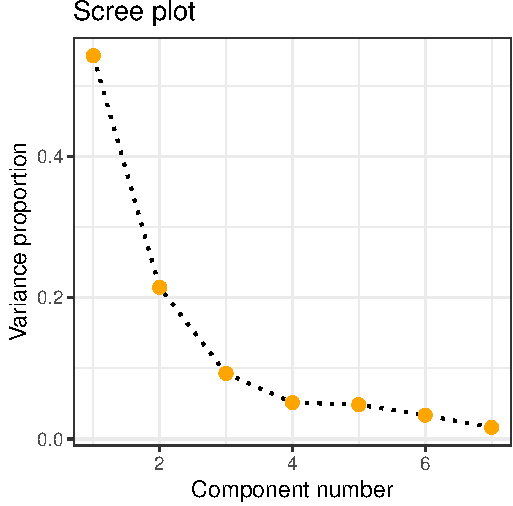
\includegraphics{sol_A2_files/figure-latex/unnamed-chunk-14-1} \end{center}

Proportion variance explained by the 1st PC is 0.54, first two is 0.76
etc.First PC is a measure of overall size of the person. Second PC
contrasts head measurements with the rest. Third PC is the head length.

\begin{enumerate}
\def\labelenumi{\arabic{enumi}.}
\setcounter{enumi}{3}
\tightlist
\item
  For each of the following situations, answer, if possible: (i) Is it a
  classification or regression problem? (ii) Are we most intererest in
  inference or prediction? (iii) Provide n and p.~For each predictor
  described state whether it is categorical or quantitative. (iv)
  Indicate whether we would expect the performance of a flexible
  learning method to be better or worse than an inflexible method.
\end{enumerate}

\begin{enumerate}
\def\labelenumi{(\alph{enumi})}
\tightlist
\item
  We have a set of data on 500 worldwide tech firms. For each firm,
  information on profit, CEO salary, number of employees, average
  employee salary, and home country is recorded. We are interested in
  the relationship between CEO salary and other measurements.
\end{enumerate}

\begin{quote}
Regression, inference, n = 500, 1 response, 4 predictors. All predictors
are quantitative, except country which is categorical. Inflexible better
for inference.
\end{quote}

\begin{enumerate}
\def\labelenumi{(\alph{enumi})}
\setcounter{enumi}{1}
\tightlist
\item
  A company wishes to launch a new product. They want to know in advance
  whether it will be a success or failure. They collect data on 20
  similar products, and record whether they succeeded or not, price
  charged, marketing budget, and 10 other variables.
\end{enumerate}

\begin{quote}
Classification, prediction, n = 20, 1 response (binary), 12 predictors.
All described predictors are quantitative. Inflexible\\
better because there are so many predictors relative to n.
\end{quote}

\begin{enumerate}
\def\labelenumi{(\alph{enumi})}
\setcounter{enumi}{2}
\tightlist
\item
  A dataset was collected to related the birthweight of babies to the
  days of gestation and gender.
\end{enumerate}

\begin{quote}
Regression, inference, n = unknown, 1 response (quantitative), 2
predictors, birthweight quantitative and gender categorical. Inflexible
better to understand predictors response association.
\end{quote}

\begin{enumerate}
\def\labelenumi{(\alph{enumi})}
\setcounter{enumi}{3}
\tightlist
\item
  Observations were collected on 56 attributes from 32 lung cancer
  patients belonging to one of 3 classes.
\end{enumerate}

\begin{quote}
Classification, prediction, n = 32, 1 response (categorical, 3 classes),
56 predictors, structure unknown. Inflexible since n is so large
relative to p.
\end{quote}

\begin{enumerate}
\def\labelenumi{\arabic{enumi}.}
\setcounter{enumi}{4}
\tightlist
\item
  In this exercise you will conduct an experiment to compare the fits on
  a linear and flexible model fit. You will use the Auto data from the
  package ISLR and explore the relationship between the response mpg
  with weight and horsepower.
\end{enumerate}

\begin{Shaded}
\begin{Highlighting}[]
\CommentTok{# install.packages("ISLR") #home computer, first time only}
\KeywordTok{library}\NormalTok{(ISLR)}
\NormalTok{auto <-}\StringTok{ }\NormalTok{Auto[}\KeywordTok{complete.cases}\NormalTok{(Auto[,}\KeywordTok{c}\NormalTok{(}\DecValTok{1}\NormalTok{,}\DecValTok{4}\NormalTok{,}\DecValTok{5}\NormalTok{)]), ] }\CommentTok{# to remove NAs}
\end{Highlighting}
\end{Shaded}

\begin{enumerate}
\def\labelenumi{(\alph{enumi})}
\tightlist
\item
  Plot the response (miles per gallon) vs weight and horsepower. What do
  they tell you about the relationship between mpg and the predictors?
\end{enumerate}

\begin{Shaded}
\begin{Highlighting}[]
\NormalTok{auto_ggplot <-}\StringTok{ }\NormalTok{auto }\OperatorTok\StringTok{ }
\StringTok{  }\KeywordTok{select}\NormalTok{(mpg, weight, horsepower) }\OperatorTok\StringTok{ }
\StringTok{  }\KeywordTok{gather}\NormalTok{(}\DataTypeTok{key =} \StringTok{"key"}\NormalTok{, }\DataTypeTok{value =} \StringTok{"value"}\NormalTok{, }\OperatorTok{-}\NormalTok{mpg)}

\NormalTok{auto_ggplot }\OperatorTok\StringTok{ }
\StringTok{  }\KeywordTok{ggplot}\NormalTok{(}\KeywordTok{aes}\NormalTok{(}\DataTypeTok{x =}\NormalTok{ value, }\DataTypeTok{y =}\NormalTok{ mpg)) }\OperatorTok{+}
\StringTok{  }\KeywordTok{facet_wrap}\NormalTok{(}\OperatorTok{~}\NormalTok{key, }\DataTypeTok{scales =} \StringTok{'free'}\NormalTok{) }\OperatorTok{+}
\StringTok{  }\KeywordTok{geom_point}\NormalTok{(}\DataTypeTok{colour =} \StringTok{"tomato"}\NormalTok{) }\OperatorTok{+}
\StringTok{  }\KeywordTok{labs}\NormalTok{(}\DataTypeTok{x =} \StringTok{"values"}\NormalTok{) }\OperatorTok{+}
\StringTok{  }\KeywordTok{theme_bw}\NormalTok{()}
\end{Highlighting}
\end{Shaded}

\begin{center}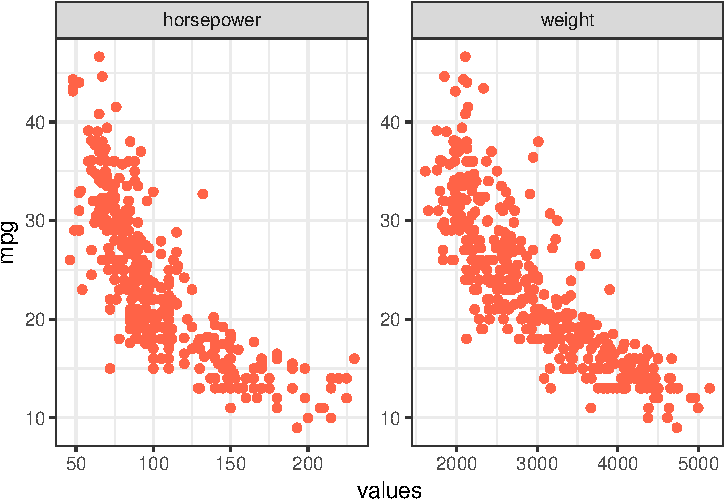
\includegraphics{sol_A2_files/figure-latex/unnamed-chunk-16-1} \end{center}

\begin{quote}
mpg goes down as weight or horsepower goes up, and both plots show
curvature.
\end{quote}

\begin{enumerate}
\def\labelenumi{(\alph{enumi})}
\setcounter{enumi}{1}
\tightlist
\item
  Make a 3d plot of weight, horsepower and mpg (see commands above).
  What do they tell you about the relationship between mpg and the
  predictors?
\end{enumerate}

\begin{Shaded}
\begin{Highlighting}[]
\KeywordTok{library}\NormalTok{(plot3D) }
\KeywordTok{library}\NormalTok{(plot3Drgl)}

\KeywordTok{scatter3D}\NormalTok{(auto}\OperatorTok{$}\NormalTok{weight, auto}\OperatorTok{$}\NormalTok{horsepower, auto}\OperatorTok{$}\NormalTok{mpg)}
\end{Highlighting}
\end{Shaded}

\begin{center}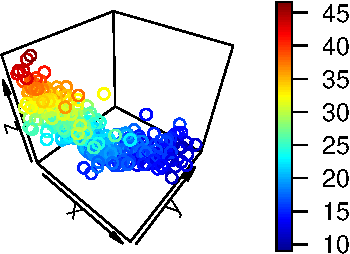
\includegraphics{sol_A2_files/figure-latex/unnamed-chunk-17-1} \end{center}

\begin{Shaded}
\begin{Highlighting}[]
\CommentTok{# scatter3Drgl(auto$weight, auto$horsepower, auto$mpg)}
\end{Highlighting}
\end{Shaded}

\begin{quote}
The plot shows that points lie on a surface, not a plane, so a linear
fit is not appropriate.
\end{quote}

\begin{enumerate}
\def\labelenumi{(\alph{enumi})}
\setcounter{enumi}{2}
\tightlist
\item
  Next, divide the data into a training set and a test set as follows:
\end{enumerate}

\begin{Shaded}
\begin{Highlighting}[]
\KeywordTok{set.seed}\NormalTok{(}\DecValTok{123}\NormalTok{)}
\NormalTok{train <-}\StringTok{ }\KeywordTok{sample}\NormalTok{(}\KeywordTok{nrow}\NormalTok{(auto), }\KeywordTok{round}\NormalTok{(}\FloatTok{0.8} \OperatorTok{*}\StringTok{ }\KeywordTok{nrow}\NormalTok{(auto)))}
\NormalTok{auto_train <-}\StringTok{ }\NormalTok{auto[train,]}
\NormalTok{auto_test <-}\StringTok{ }\NormalTok{auto[}\OperatorTok{-}\NormalTok{train,]}
\end{Highlighting}
\end{Shaded}

Fit a linear regression model to mpg versus weight and horsepower on
AutoTrain. Call the fit f1. Examine summary(f1) and comment on the
significance of the predictors.

\begin{Shaded}
\begin{Highlighting}[]
\NormalTok{f1 <-}\StringTok{ }\KeywordTok{lm}\NormalTok{(mpg }\OperatorTok{~}\NormalTok{weight }\OperatorTok{+}\StringTok{ }\NormalTok{horsepower, }\DataTypeTok{data =}\NormalTok{ auto_train)}
\KeywordTok{summary}\NormalTok{(f1)}
\end{Highlighting}
\end{Shaded}

\begin{verbatim}
## 
## Call:
## lm(formula = mpg ~ weight + horsepower, data = auto_train)
## 
## Residuals:
##      Min       1Q   Median       3Q      Max 
## -11.4101  -2.7431  -0.4644   2.5079  16.0258 
## 
## Coefficients:
##               Estimate Std. Error t value Pr(>|t|)    
## (Intercept) 46.1626326  0.8950964   51.57  < 2e-16 ***
## weight      -0.0060579  0.0005553  -10.91  < 2e-16 ***
## horsepower  -0.0431712  0.0120932   -3.57 0.000414 ***
## ---
## Signif. codes:  0 '***' 0.001 '**' 0.01 '*' 0.05 '.' 0.1 ' ' 1
## 
## Residual standard error: 4.339 on 311 degrees of freedom
## Multiple R-squared:  0.7087, Adjusted R-squared:  0.7068 
## F-statistic: 378.3 on 2 and 311 DF,  p-value: < 2.2e-16
\end{verbatim}

\begin{enumerate}
\def\labelenumi{(\alph{enumi})}
\setcounter{enumi}{3}
\tightlist
\item
  Plot the fitted surface and the data. (See lecture notes for code).
  Does the linear surface look like a good fit?
\end{enumerate}

\begin{Shaded}
\begin{Highlighting}[]
\NormalTok{wt1 <-}\StringTok{ }\KeywordTok{seq}\NormalTok{(}\DecValTok{1610}\NormalTok{, }\DecValTok{5140}\NormalTok{, }\DataTypeTok{length.out =} \DecValTok{30}\NormalTok{)}
\NormalTok{hp1 <-}\StringTok{ }\KeywordTok{seq}\NormalTok{(}\DecValTok{45}\NormalTok{, }\DecValTok{230}\NormalTok{, }\DataTypeTok{length.out =} \DecValTok{30}\NormalTok{)}
\NormalTok{pred <-}\StringTok{ }\KeywordTok{predict}\NormalTok{(f1, }\KeywordTok{expand.grid}\NormalTok{(}\DataTypeTok{weight =}\NormalTok{ wt1, }\DataTypeTok{horsepower =}\NormalTok{ hp1))}
\NormalTok{pred <-}\StringTok{ }\KeywordTok{matrix}\NormalTok{(pred, }\DecValTok{30}\NormalTok{, }\DecValTok{30}\NormalTok{)}

\KeywordTok{scatter3D}\NormalTok{(auto_train}\OperatorTok{$}\NormalTok{weight, auto_train}\OperatorTok{$}\NormalTok{horsepower, auto_train}\OperatorTok{$}\NormalTok{mpg, }
          \DataTypeTok{pch =} \DecValTok{18}\NormalTok{, }\DataTypeTok{surf =} \KeywordTok{list}\NormalTok{(}\DataTypeTok{x =}\NormalTok{ wt1, }\DataTypeTok{y =}\NormalTok{ hp1, }\DataTypeTok{z =}\NormalTok{ pred))}
\end{Highlighting}
\end{Shaded}

\begin{center}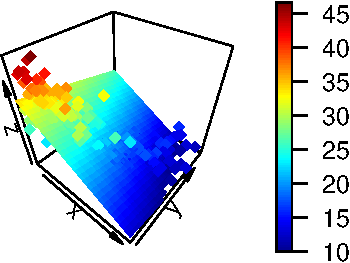
\includegraphics{sol_A2_files/figure-latex/unnamed-chunk-20-1} \end{center}

\begin{quote}
We can see that for high values of z = mpg, points lie far away and
mostly above from the fitted planes so the linear fit does not look
appropriate.
\end{quote}

\begin{enumerate}
\def\labelenumi{(\alph{enumi})}
\setcounter{enumi}{4}
\tightlist
\item
  Use loess to fit a surface to the same data. Call the fit f2. Plot the
  fitted surface and the data. Does the loess surface look like a good
  fit?
\end{enumerate}

\begin{Shaded}
\begin{Highlighting}[]
\NormalTok{f2 <-}\StringTok{ }\KeywordTok{loess}\NormalTok{(mpg }\OperatorTok{~}\StringTok{ }\NormalTok{weight }\OperatorTok{+}\StringTok{ }\NormalTok{horsepower, }\DataTypeTok{data =}\NormalTok{ auto_train)}
\NormalTok{pred <-}\StringTok{ }\KeywordTok{predict}\NormalTok{(f2, }\KeywordTok{expand.grid}\NormalTok{(}\DataTypeTok{weight =}\NormalTok{ wt1, }\DataTypeTok{horsepower =}\NormalTok{ hp1))}
\NormalTok{pred <-}\StringTok{ }\KeywordTok{matrix}\NormalTok{(pred,}\DecValTok{30}\NormalTok{,}\DecValTok{30}\NormalTok{)}

\KeywordTok{scatter3D}\NormalTok{(auto_train}\OperatorTok{$}\NormalTok{weight,auto_train}\OperatorTok{$}\NormalTok{horsepower,auto_train}\OperatorTok{$}\NormalTok{mpg, }
          \DataTypeTok{pch =} \DecValTok{18}\NormalTok{, }\DataTypeTok{surf =} \KeywordTok{list}\NormalTok{(}\DataTypeTok{x =}\NormalTok{ wt1, }\DataTypeTok{y =}\NormalTok{ hp1, }\DataTypeTok{z =}\NormalTok{ pred))}
\end{Highlighting}
\end{Shaded}

\begin{center}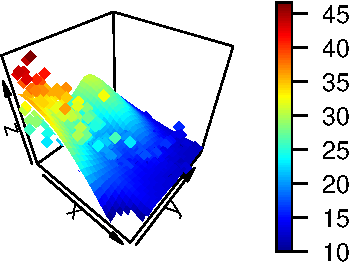
\includegraphics{sol_A2_files/figure-latex/unnamed-chunk-21-1} \end{center}

\begin{quote}
Now it looks like we captured the pattern of the association, but a
smoother surface might be better.
\end{quote}

\begin{enumerate}
\def\labelenumi{(\alph{enumi})}
\setcounter{enumi}{5}
\tightlist
\item
  Calculate the MSE for both fits on the training data. What do these
  numbers tell you?
\end{enumerate}

\begin{Shaded}
\begin{Highlighting}[]
\KeywordTok{mean}\NormalTok{(}\KeywordTok{residuals}\NormalTok{(f1)}\OperatorTok{^}\DecValTok{2}\NormalTok{)}
\end{Highlighting}
\end{Shaded}

\begin{verbatim}
## [1] 18.64557
\end{verbatim}

\begin{Shaded}
\begin{Highlighting}[]
\KeywordTok{mean}\NormalTok{(}\KeywordTok{residuals}\NormalTok{(f2)}\OperatorTok{^}\DecValTok{2}\NormalTok{)}
\end{Highlighting}
\end{Shaded}

\begin{verbatim}
## [1] 16.12921
\end{verbatim}

\begin{quote}
The train MSE for the flexible model is smaller.
\end{quote}

\begin{enumerate}
\def\labelenumi{(\alph{enumi})}
\setcounter{enumi}{6}
\tightlist
\item
  Calculate the MSE for both fits on the test data. What do these
  numbers tell you?
\end{enumerate}

\begin{Shaded}
\begin{Highlighting}[]
\NormalTok{pred1 <-}\StringTok{ }\KeywordTok{predict}\NormalTok{(f1, auto_test)}
\KeywordTok{mean}\NormalTok{((pred1 }\OperatorTok{-}\StringTok{ }\NormalTok{auto_test}\OperatorTok{$}\NormalTok{mpg)}\OperatorTok{^}\DecValTok{2}\NormalTok{)}
\end{Highlighting}
\end{Shaded}

\begin{verbatim}
## [1] 14.81678
\end{verbatim}

\begin{Shaded}
\begin{Highlighting}[]
\NormalTok{pred2 <-}\StringTok{ }\KeywordTok{predict}\NormalTok{(f2, auto_test)}
\KeywordTok{mean}\NormalTok{((pred2 }\OperatorTok{-}\StringTok{ }\NormalTok{auto_test}\OperatorTok{$}\NormalTok{mpg)}\OperatorTok{^}\DecValTok{2}\NormalTok{)}
\end{Highlighting}
\end{Shaded}

\begin{verbatim}
## [1] 14.70665
\end{verbatim}

\begin{quote}
The test MSE is about the same for both fits: choose the simpler model
(OLS).
\end{quote}


\end{document}
